\documentclass[a4paper,12pt]{article}
\usepackage[utf8]{inputenc}
\usepackage{xcolor}
\usepackage{url}
\usepackage[T2A]{fontenc}
\usepackage{graphicx}
\usepackage[margin=80pt]{geometry}

\usepackage[english,serbian]{babel}

\begin{document}

\newpage
\section{Margaret Hamilton}

\begin{flushleft}
 Margaret Hamilton (rođena 17. avgusta 1936, Paoli, Indijana, SAD), američki informatičar koji je bio jedan od prvih programera kompjuterskog softvera; stvorila je termin softverski inženjer da opiše svoj rad. Pomogla je u pisanju kompjuterskog koda za komandne i lunarne module korišćene u misijama Apolo na Mesec kasnih 1960-ih i ranih 70-ih.

    Studirala je matematiku i filozofiju na Earlham koledžu u Ričmondu, Indijana. Nakon diplomiranja 1958. kratko je predavala matematiku u srednjoj školi. Iako je Margaret planirala da studira apstraktnu matematiku na Univerzitetu Brandeis, prihvatila je posao na Tehnološkom institutu u Masačusetsu (MIT) dok je njen suprug pohađao Pravni fakultet Harvarda. Na MIT-u je počela da programira softver za predviđanje vremena i radila je na postdiplomskim studijama iz meteorologije.
    Početkom 1960-ih Hamiltonova se pridružila MIT-ovoj Lincoln laboratoriji, gde je bila uključena u projekat Poluautomatsko zemaljsko okruženje (SAGE), prvi američki sistem protivvazdušne odbrane. Posebno je napisala softver za program za identifikaciju neprijateljskih aviona. Hamilton je zatim radila u MIT-ovoj laboratoriji za instrumentaciju (sada nezavisna laboratorija Charles Stark Draper), koja je obezbedila aeronautičku tehnologiju za Nacionalnu upravu za aeronautiku i svemir (NASA). Predvodila je tim koji je imao zadatak da razvije softver za sisteme navođenja i kontrole komandnih i lunarnih modula misija Apolo u letu. U to vreme nijedna škola nije predavala softversko inženjerstvo, tako da su članovi tima morali sami da rešavaju probleme. Ona je kreirala termin softverski inženjer jer je smatrala da je posao koji ona i njen tim obavljaju jednako važan i jednako inženjerski kao i drugi rad na svemirskoj letelici Apolo. Sama Margaret se posebno koncentrisala na softver za otkrivanje sistemskih grešaka i za oporavak informacija u slučaju pada računara. Oba ta elementa bila su presudna tokom misije Apolo 11 (1969), koja je odvela astronaute Nila Armstronga i Baza Oldrina na Mesec. Hamilton je napustila MIT sredinom 1970-ih da bi radio u privatnom sektoru. Suosnivala je kompaniju Higher Order Softvare 1976. godine i osnovala Hamilton Technologies 10 godina kasnije.

    Hamilton je bila dobitnica raznih počasti, uključujući NASA-ina nagradu o izuzetnom dostignucu.
    
    
    \begin{figure}[h]
    \centering
    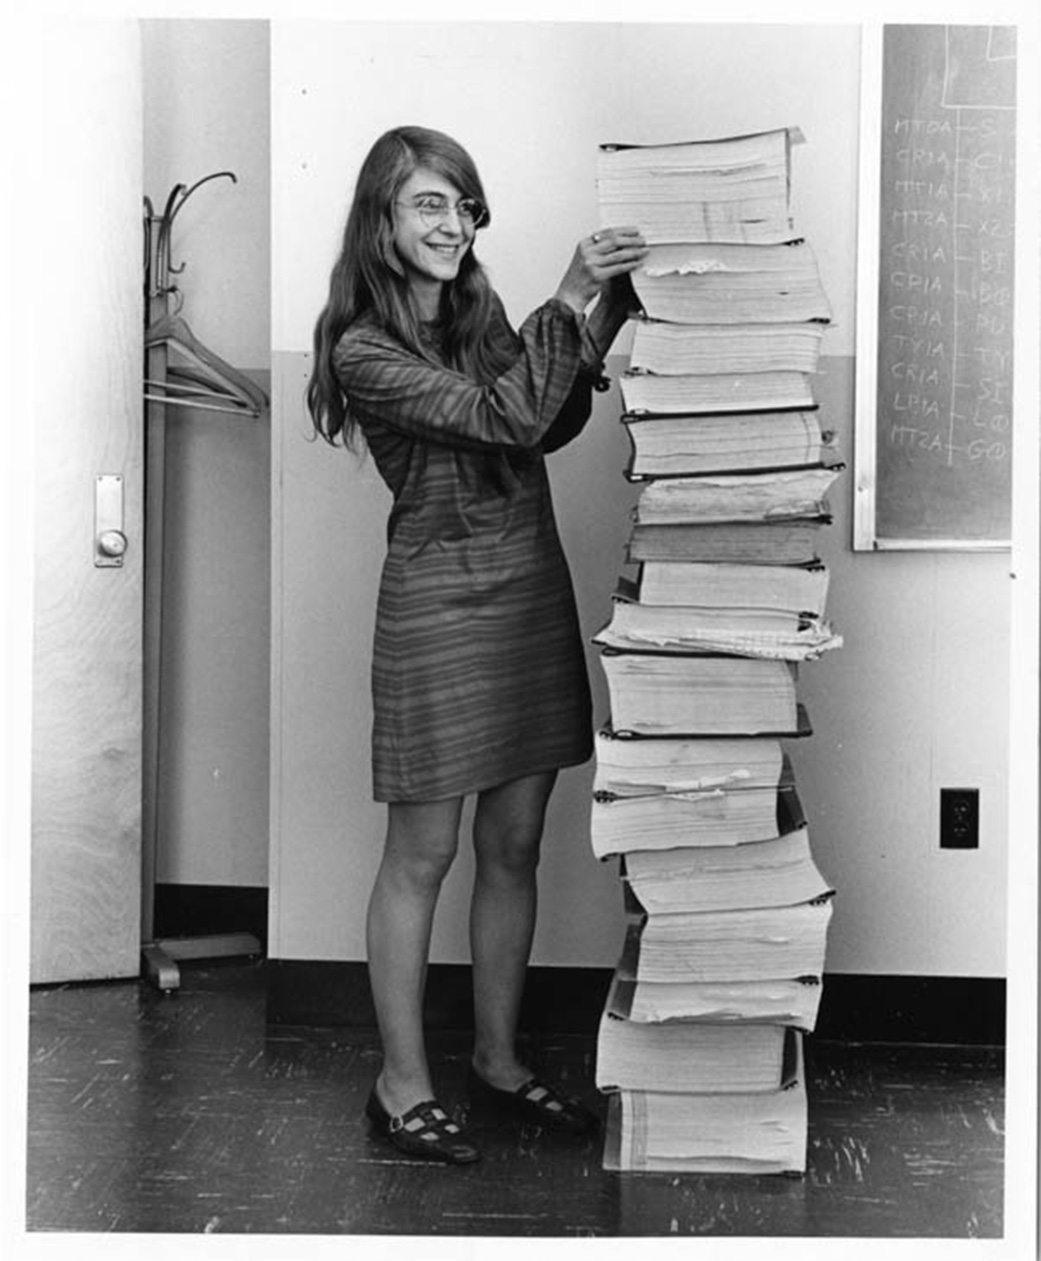
\includegraphics[width = .6\textwidth]{margaret_hamilton5.jpg}
    \caption{Margaret Hamilton}
    \label{fig:my_label}
\end{figure}




\end{document}
